%%%%%%%%%%%%%%
%% Run LaTeX on this file several times to get Table of Contents,
%% cross-references, and citations.

%% If you have font problems, you may edit the w-bookps.sty file
%% to customize the font names to match those on your system.

%% w-bksamp.tex. Current Version: Feb 16, 2012
%%%%%%%%%%%%%%%%%%%%%%%%%%%%%%%%%%%%%%%%%%%%%%%%%%%%%%%%%%%%%%%%
%
%  Sample file for
%  Wiley Book Style, Design No.: SD 001B, 7x10
%  Wiley Book Style, Design No.: SD 004B, 6x9
%
%
%  Prepared by Amy Hendrickson, TeXnology Inc.
%  http://www.texnology.com
%%%%%%%%%%%%%%%%%%%%%%%%%%%%%%%%%%%%%%%%%%%%%%%%%%%%%%%%%%%%%%%%

%%%%%%%%%%%%%
% 7x10
%\documentclass{wileySev}

% 6x9
\documentclass{wileySix}

\usepackage{graphicx}
\usepackage{listings}

\usepackage{color}
 
\definecolor{codegreen}{rgb}{0,0.6,0}
\definecolor{codegray}{rgb}{0.5,0.5,0.5}
\definecolor{codepurple}{rgb}{0.58,0,0.82}
\definecolor{backcolour}{rgb}{0.95,0.95,0.92}
 
\lstdefinestyle{mystyle}{
    backgroundcolor=\color{backcolour},   
    commentstyle=\color{codegreen},
    keywordstyle=\color{magenta},
    numberstyle=\tiny\color{codegray},
    stringstyle=\color{codepurple},
    basicstyle=\footnotesize,
    breakatwhitespace=false,         
    breaklines=true,                 
    captionpos=b,                    
    keepspaces=true,                 
    numbers=left,                    
    numbersep=5pt,                  
    showspaces=false,                
    showstringspaces=false,
    showtabs=false,                  
    tabsize=2,
    language=sh
}
 
\lstset{style=mystyle}

%%%%%%%
%% for times math: However, this package disables bold math (!)
%% \mathbf{x} will still work, but you will not have bold math
%% in section heads or chapter titles. If you don't use math
%% in those environments, mathptmx might be a good choice.

% \usepackage{mathptmx}

% For PostScript text
\usepackage{w-bookps}

%%%%%%%%%%%%%%%%%%%%%%%%%%%%%%%%%%%%%%%%%%%%%%%%%%%%%%%%%%%%%%%%
%% Other packages you might want to use:

% for chapter bibliography made with BibTeX
% \usepackage{chapterbib}

% for multiple indices
% \usepackage{multind}

% for answers to problems
% \usepackage{answers}

%%%%%%%%%%%%%%%%%%%%%%%%%%%%%%
%% Change options here if you want:
%%
%% How many levels of section head would you like numbered?
%% 0= no section numbers, 1= section, 2= subsection, 3= subsubsection
%%==>>
\setcounter{secnumdepth}{3}

%% How many levels of section head would you like to appear in the
%% Table of Contents?
%% 0= chapter titles, 1= section titles, 2= subsection titles, 
%% 3= subsubsection titles.
%%==>>
\setcounter{tocdepth}{2}

%% Cropmarks? good for final page makeup
%% \docropmarks

%%%%%%%%%%%%%%%%%%%%%%%%%%%%%%
%
% DRAFT
%
% Uncomment to get double spacing between lines, current date and time
% printed at bottom of page.
% \draft
% (If you want to keep tables from becoming double spaced also uncomment
% this):
% \renewcommand{\arraystretch}{0.6}
%%%%%%%%%%%%%%%%%%%%%%%%%%%%%%

%%%%%%% Demo of section head containing sample macro:
%% To get a macro to expand correctly in a section head, with upper and
%% lower case math, put the definition and set the box 
%% before \begin{document}, so that when it appears in the 
%% table of contents it will also work:

\newcommand{\VT}[1]{\ensuremath{{V_{T#1}}}}

%% use a box to expand the macro before we put it into the section head:

\newbox\sectsavebox
\setbox\sectsavebox=\hbox{\boldmath\VT{xyz}}

%%%%%%%%%%%%%%%%% End Demo


\begin{document}


\booktitle{Cerdas Menguasai Python}
\subtitle{Dalam 24 Jam}

\authors{Rolly M. Awangga\\
\affil{Informatics Research Center}
%Floyd J. Fowler, Jr.\\
%\affil{University of New Mexico}
}

\offprintinfo{Cerdas Menguasai Python, First Edition}{Rolly M. Awangga}

%% Can use \\ if title, and edition are too wide, ie,
%% \offprintinfo{Survey Methodology,\\ Second Edition}{Robert M. Groves}

%%%%%%%%%%%%%%%%%%%%%%%%%%%%%%
%% 
\halftitlepage

\titlepage


\begin{copyrightpage}{2019}
%Survey Methodology / Robert M. Groves . . . [et al.].
%\       p. cm.---(Wiley series in survey methodology)
%\    ``Wiley-Interscience."
%\    Includes bibliographical references and index.
%\    ISBN 0-471-48348-6 (pbk.)
%\    1. Surveys---Methodology.  2. Social 
%\  sciences---Research---Statistical methods.  I. Groves, Robert M.  II. %
%Series.\\
%
%HA31.2.S873 2007
%001.4'33---dc22                                             2004044064
\end{copyrightpage}

\dedication{`Jika Kamu tidak dapat menahan lelahnya belajar, 
Maka kamu harus sanggup menahan perihnya Kebodohan.'
~Imam Syafi'i~}

\begin{contributors}
\name{Rolly Maulana Awangga,} Informatics Research Center., Politeknik Pos Indonesia, Bandung,
Indonesia



\end{contributors}

\contentsinbrief
\tableofcontents
\listoffigures
\listoftables
\lstlistoflistings


\begin{foreword}
Sepatah kata dari Kaprodi, Kabag Kemahasiswaan dan Mahasiswa
\end{foreword}

\begin{preface}
Buku ini diciptakan bagi yang awam dengan git sekalipun.

\prefaceauthor{R. M. Awangga}
\where{Bandung, Jawa Barat\\
Februari, 2019}
\end{preface}


\begin{acknowledgments}
Terima kasih atas semua masukan dari para mahasiswa agar bisa membuat buku ini 
lebih baik dan lebih mudah dimengerti.

Terima kasih ini juga ditujukan khusus untuk team IRC yang 
telah fokus untuk belajar dan memahami bagaimana buku ini mendampingi proses 
Intership.
\authorinitials{R. M. A.}
\end{acknowledgments}

\begin{acronyms}
\acro{ACGIH}{American Conference of Governmental Industrial Hygienists}
\acro{AEC}{Atomic Energy Commission}
\acro{OSHA}{Occupational Health and Safety Commission}
\acro{SAMA}{Scientific Apparatus Makers Association}
\end{acronyms}

\begin{glossary}
\term{git}Merupakan manajemen sumber kode yang dibuat oleh linus torvald.

\term{bash}Merupakan bahasa sistem operasi berbasiskan *NIX.

\term{linux}Sistem operasi berbasis sumber kode terbuka yang dibuat oleh Linus Torvald
\end{glossary}

\begin{symbols}
\term{A}Amplitude

\term{\hbox{\&}}Propositional logic symbol 

\term{a}Filter Coefficient

\bigskip

\term{\mathcal{B}}Number of Beats
\end{symbols}

\begin{introduction}

%% optional, but if you want to list author:

\introauthor{Rolly Maulana Awangga, S.T., M.T.}
{Informatics Research Center\\
Bandung, Jawa Barat, Indonesia}

Pada era disruptif  \index{disruptif}\index{disruptif!modern} 
saat ini. git merupakan sebuah kebutuhan dalam sebuah organisasi pengembangan perangkat lunak.
Buku ini diharapkan bisa menjadi penghantar para programmer, analis, IT Operation dan Project Manajer.
Dalam melakukan implementasi git pada diri dan organisasinya.

Rumusnya cuman sebagai contoh aja biar keren\cite{awangga2018sampeu}.

\begin{equation}
ABC {\cal DEF} \alpha\beta\Gamma\Delta\sum^{abc}_{def}
\end{equation}

\end{introduction}

%%%%%%%%%%%%%%%%%%Isi Buku_

\chapter{Judul Bagian Pertama}
\section{Irvan Rizkiansyah}

\section{Python}
	\subsection{Background}
	\label{Background}
	\par
	Python adalah sebuah bahasa pemrograman yang bersifat interpreter, interactive, object-oriented, dan dapat beroperasi hampir pada semua platform seperti Windows, Linux, Mac. Python termasuk sebagai bahasa pemrograman yang dapat dengan mudah di pelajari karena sintaks yang jelas dan mudah dipahami, dan dapat dikombinasikan dengan penggunaan modul yang siap pakai, dan struktur data tingkat tinggi yang efisien \cite{prasetya2012deteksi}.
	\par
	Python memiliki kepustakaan atau biasa disebut library yang sangat luas, dan dalam distribusi Python yang telah disediakan, hal tersebut diakibatkan oleh pendistribusian Python yang bebas karena bahasa pemrograman Python merupakan bahasa pemrograman yang freeware atau bebas dalam hal pengembangannya. Python adalah sebuah bahasa pemrograman yang dapat dengan mudah dibaca dan terstruktur, hal tersebut dikarenakan penggunaan sistem identasi, yaitu pemisahan blok-blok program susunan identasi, jadi untuk menambahkan sub-sub program dalam sebuah blok program, sub program tersebut harus diletakkan pada satu atau lebih spasi dari kolom sebuah blok \cite{perkasa2014rancang}.
	\par
	Bahasa pemrograman Python dibuat oleh Guido Van Rossum. Dikarenakan para pengembang software atau perangkat lunak lebih cenderung memilih kecepatan dalam menyelesaikan suatu proyek dibandingkan dengan kecepatam proses dari program yang dijalankan, maka dari itu bahasa pemrograman Python dapat dibilang bahasa pemerograman yang kecepatannya dapat melebihi bahasa pemrograman C. Akan tetapi bahasa pemrograman Python lebih lambat dalam memproses suatu program dibandingkan bahasa pemrograman C. dengan berkembangnya kecepatan prosesor dan memori saat ini, mengakibatkan tidak terlihatnya keterlambatan dari sebuah program yang menggunakan bahasa pemrograman Python \cite{miftakhuddinimplementasi}.

	\subsection{Problems}
		\begin{itemize}
			\item Kurangnya pemahaman tentang bahasa pemrograman Python
			\item Kurang mengerti dalam hal fungsi-fungsi yang terdapat pada bahasa pemrograman Python
		\end{itemize}

	\subsection{Objective and Contribution}
		\subsubsection{Objective}
			\begin{itemize}
				\item Dapat memahami tentang bahasa pemrograman Python
				\item Dapat memahami fungsi fungsi yang terdapat pada bahasa pemrograman Python
			\end{itemize}
	
		\subsubsection{Contribution}
			\begin{itemize}
				\item Dapat membangun sebuah sistem dengan menggunakan bahasa pemrograman Python
				\item Dapat membangun sebuah alat yang berguna, menggunakan mikrokontroler dan bahasa pemrograman python
			\end{itemize}

	\subsection{Scoop and Environtment}
		\begin{itemize}
			\item Pengenanalan tentang bahasa pemrograman Python
			\item Pengenalan fungsi-fungsi yang terdapat pada bahasa pemrograman Python
		\end{itemize}

\section{Luthfi Muhammad Nabil\_1174035}
\subsection{Background}
Python adalah sebuah bahasa pemrograman dengan level tinggi yang interaktif, dan mendukung berbagai paradigma pemrograman. Python sudah terkenal pada kalangan programmer sebagai bahasa yang mudah dipahami dan memiliki kompleksitas yang dinamis sehingga dapat dipakai di algoritma maupun platform yang berbagai macam.Python sudah memiliki banyak komunitas pendukung karena penggunanya yang banyak. Selain pada komunitas biasa, Python sudah diimplementasikan pada banyak perusahaan ternama dan dipasang pada aplikasi yang sudah terkenal seperti pada search engine google yang dimiliki oleh perusahaan Google. 
\linebreak
\linebreak
Python mulai dirilis pada tahun 1991 oleh Guido van Rossum sebagai kelanjutan dari bahasa pemrograman ABC dengan memiliki versi yaitu 0.9.0. Nama dari bahasa Python diambil dari program televisi di Inggris bernama Monty Python. Lalu tahun 1995, Guido pindah ke CNRI di Virginia, Amerika sembari melanjutkan pengembangan Python. Versi terakhir yang dikeluarkan telah mencapai 1.6. Pada awalnya, Python adalah bahasa yang dipakai untuk  Lalu pada tahun 2000, dirilis Python versi 2.0 yang memiliki peran sebagai bahasa pemrograman tidak berbayar atau open source. Van Rossum sendiri aktif pada development dari Python tetapi sudah bergabung dengan banyak penyumbang. Dibandingkan dengan bahasa lain, Python sudah melewati beberapa versi yang terbatas, mengikuti filosofi dari perubahan berurutan. 
\linebreak
\linebreak
Untuk memahami bahasa Python tidak sulit, tetapi instalasi Python cukup memiliki trik tersendiri terlebih untuk pengguna yang baru memasuki lingkup programming. Pada sistem operasi windows, pengguna diharuskan untuk memasuki sistem pada windows untuk mengatur lokasi dari Python yang sudah diinstall. Selain itu, untuk yang terbiasa dengan beberapa pemrograman harus beradaptasi dengan aturan - aturan pada bahasa pemrograman Python seperti penggantian titik koma (;) dengan indentasi. Oleh karena itu, penulis akan membahas mengenai pengenalan singkat mengenai bahasa pemrograman python dan cara instalasi dari python dan library pip.

\subsection{Problems}
Sesuai dengan latar belakang yang telah dibahas, penulis merumuskan masalah sebagai berikut : 
\begin{enumerate}	
	\item Bagaimana pemaparan singkat mengenai Python?
	\item Bagaimana cara melakukan instalasi Python?
\end{enumerate}

\subsection{Objective and Contribution}
\subsubsection{Objective}
\begin{enumerate}
	\item Untuk membahas mengenai Python.
	\item Untuk menunjukkan cara instalasi Python.
\end{enumerate}

\subsubsection{Contribution}
Pada materi ini, penulis menggunakan Python.

\subsection{Scoop and Environment}
\begin{itemize}
	\item Pada Chapter 1 membahas mengenai sejarah, latar belakang, dan keterangan singkat mengenai python tersebut. Chapter ini juga merangkum masalah dan mencari tujuan yang ingin dicapai penulis dalam membuat resume ini.
\end{itemize}

\section{Hagan Rowlenstino/1174040}
\subsection{Background}
Python di desain sebagai bahasa pemrograman yang dapat digunakan sehari-hari. Pencipta python ,Guido van Rossum, telah menulis seri lengkap tentang sejarah bahasa tersebut.Python diciptakan di awal 1990 di CWI \'(the Centrum voor Wiskunde and Informatica), tempat kelahiran ALGOL \'(Algorithmic Language 68 ). Sebelumnya, Rossum juga telah mengerjakan bahasa pemrograman ABC, yang dikembangkan di  CWI sebagai bahasa pengajaran yang menekankan kejelasan. Walaupun project ABC telah di tutup , Rossum banyak belajar dari hal tersebut saat dia mulai membuat Python sebagai alat untuk multimedia dan project penelitian sistem operasi. Dia ingin Python mempunyai tingkatan yang cukup tinggi agar mudah untuk dibaca dan ditulis, juga mirip dengan Java, dan menawarkan portabilitas serta error model yang terdefinisi dengan baik.
\linebreak
\linebreak
Python juga kaya akan vocabulary yang berguna untuk membuat algoritma yang kompleks dengan efisien dikarenakan punya dictionaries yang memiliki string yang kuat dan assosiasi array yang fleksibel. Python menggabungkan antara fleksibilitas tingkat tinggi, kemampuan membaca, dan interface yang terdefinisi dengan baik. Kombinasi tersebut membuat Python cocok untuk menyelesaikan masalah komputasi non-algoritma seperti integrase dengan web, format data, ataw hardware kelas rendah. Python mudah untuk dipelajari karena strukturnya sederhana dan sintaksnya jelas, punya library yang portable dan dapat digunakan di beda perangkat,dan dapat terintegrasi dengan bahasa pemrograman lain seperti C, C++, dan Java.
\subsection{Problems}
\begin{enumerate}
\item Banyak pemrograman yang penggunaannya kompleks
\end{enumerate}
\subsection{Objective and Contribution}
\subsubsection{Objective}
\begin{enumerate}
\item Dapat memudahkan pemrograman dengan bahasa pemrograman yang tepat
\end{enumerate}
\subsubsection{Contribution}
\begin{enumerate}
\item Menggunakan Python sebagai bahasa pemrograman
\end{enumerate}
\subsection{Scoop and Environment}
\begin{enumerate}
\item Mengimplementasikan Python dalam pemrograman
\end{enumerate}


\section{Faisal Najib Abdullah 1174042}
\subsection{Background}
\label{Background}
\par
Python lahir pada akhir tahun 1980-an dan implementasinya dimulai pada Desember 1989 oleh Guido van Rossum di CWI di Belanda sebagai penerus bahasa ABC (itu sendiri terinspirasi oleh SETL) yang mampu menangani pengecualian dan berinteraksi dengan sistem operasi Amuba. Van Rossum adalah penulis utama Python, dan peran sentralnya yang berkelanjutan dalam menentukan arah Python tercermin dalam judul yang diberikan kepadanya oleh komunitas Python, Benevolent Dictator for Life (BDFL).
\par
Python adalah bahasa pemrograman interpretatif multiguna dengan filosofi desain yang berfokus pada keterbacaan kode dan python sendiri diklaim sebagai bahasa yang menggabungkan kapabilitas, kemampuan, dengan kode sintaksis yang sangat jelas, dan dilengkapi dengan fungsi pustaka standar yang besar dan komprehensif. Python juga didukung oleh komunitas besar.
\par
Python mendukung pemrograman multi-paradigma, terutama tetapi tidak terbatas pada pemrograman berorientasi objek, pemrograman imperatif, dan pemrograman fungsional. Salah satu fitur yang tersedia di Python adalah sebagai bahasa pemrograman dinamis yang dilengkapi dengan manajemen memori otomatis. Python menggunakan bahasa bahasa scripting yang sama seperti bahasa pemrograman dinamis, meskipun dalam praktiknya penggunaan bahasa ini lebih luas mencakup konteks penggunaan yang umumnya tidak dilakukan menggunakan bahasa skrip. Python dapat digunakan untuk keperluan pengembangan perangkat lunak dan dapat berjalan di berbagai platform sistem operasi.
\par
CPython, implementasi referensi Python, adalah perangkat lunak bebas dan open source dan memiliki model pengembangan berbasis komunitas, seperti halnya hampir semua implementasi alternatifnya. CPython dikelola oleh Yayasan Perangkat Lunak Python nirlaba \cite{van2007python}.

\subsection{Problems}
\begin{itemize}
	\item Mahasiswa D4 TI belum dapat belum memahami apa itu python
    \item Mahasiswa D4 TI belum mengerti fungsi fungsi apa saja yang terdapat pada python
    \item Mahasiswa D4 TI belum dapat menjalankan fungsi python
\end{itemize}

\subsection{Objective and Contribution}
\subsubsection{Objective}
\begin{itemize}
	\item Mahasiswa D4 TI dapat memahami apa itu python
	\item Mahasiswa D4 TI dapat memahami fungsi fungsi yang terdapat pada python
	\item Mahasiswa D4 TI dapat menjalankan fungsi python
\end{itemize}
	
\subsubsection{Contribution}
\begin{itemize}
	\item Mahasiswa D4 TI dapat membangun suatu aplikasi yang mengimplementasikan bahasa python
	\item Mahasiswa D4 TI dapat membangun alat yang terhubung dengan aplikasi menggunakan bahasa python
\end{itemize}

\subsection{Scoop and Environtment}
\begin{itemize}
	\item Mengenali apa itu python pada mahasiswa
	\item Mengenali fungsi fungsi dasar python dan menjalankannya
\end{itemize}


\section{Ichsan Hizman Hardy/1174034}
\subsection{Background}
\par
Python merupakan bahasa pemrograman interpretatif multiguna. Python pertama kali diciptakan oleh Guido van Rossum di Stichting Mathematisch Centrum atau CWI di Belanda pada tahun 1990. pada tahun 1995, Guido melanjutkan karyanya pada Python di Virginia, dimana ia telah meliris beberapa versi perangkat lunak\cite{priyahita2015analisis}.
Tidak seperti bahasa lain yang sulit dibaca dan dipahami, python menekankan keterbacaan kode untuk membuatnya lebih mudah untuk memahami sintaksis\cite{cokelaer2013bioservices}.Ini membuat Python sangat mudah dipelajari untuk pemula dan mereka yang telah menguasai bahasa pemrograman lain.
\par
Python dengan desian yang sangat mudah di baca dan dipahami, karena sama seperti bahasa pemrograman yang lainnya yaitu dengan menggunakan bahasa inggris. selain itu juga lebih sedikit dalam penggunaan rumus atau syntac\cite{nur2018prototipe}.
\par
Pyton juga mendukung sistem teknik pemrograman yang merangkum kode dalam objek. Bahasa Python  mendukung hampir  semua sistem operasi, termasuk operasi Linux\cite{muzawi2018penerapan}.
\par
Dengan kode yang simpel dan mudah diimplementasikan, seorang programer dapat lebih mengutamakan pengembangan aplikasi yang dibuat.
	
\subsection{Problems}
\begin{enumerate}
	\item Mahasiswa D4TI2B belum bisa menggunakan bahasa python.
	\item Bagaimana pengaruh bahasa python terhadap mahasiswa D4TI2B.
	\item Bagaimana penggunaan bahasa python terhadap web service.
\end{enumerate}
	
\subsection{Objective and Contribution}
\subsubsection{Objective}
\begin{enumerate}
	\item Mahasiswa D4TI2B mampu memahami bahasa pemrograman python secara bertahap.
	\item Bahasa pemrograman python mampu mempengaruhi mahasiswa D4TI2B menjadi lebih semangat dalam belajar web service.
	\item Penggunaan bahasa python mampu mempermudah mahasiswa dalam membuat web service.
\end{enumerate}
\subsubsection{Contribution}
\begin{enumerate}
	\item Membantu mahasiswa D4TI2B dalam menyelesaikan masalah pada python.
	\item Membantu mahasiswa D4TI2B memahami bahasa pemrograman python.
	\item Mempelajari bahasa python dalam proses pembuatan web service.
\end{enumerate}
		
\subsection{Scope and Environtment}
\begin{enumerate}
	\item Mahasiswa D4TI2B memahami bahasa pemrograman python.
	\item Mahasiswa D4TI2B mampu menjalankan fungsi python.
	\item Mahasiswa D4TI2B mampu membuat web service menggunakan python.
\end{enumerate}


\chapter{Judul Bagian Kedua}

\section{IrvanRizkiansyah/1174043}
	\subsection{Teori}
		\begin{enumerate}
			\item Pada python variabel tidak perlu dideklarasikan, pendeklarasian terjadi secara otomatis pada saat memberikan suatu nilai atau data ke variabel. Terdapat beberapa jenis tipe data variabel pada python, diantaranya :
				\begin{itemize}
					\item Python Numbers, dimana akan menyimpan data yang berupa angka. Penggunaan pada python sebagai berikut : 
					var1 = 5
					var2 = 48.9
					
					\item Python Text, dimana akan menyimpan data yang berupa teks ataupun karakter. Penggunaan pada python harus diapitkan oleh tanda petik ("..."), contohnya :
					nama = "Irvan"
					jnskelamin = "L"
					
					\item Python Boolean, dimana yang hanya memiliki 2 nilai yaitu True dan False saja. penggunaan pada python huruf pertama harus kapital, contohnya :
					var3 = True
					var4 = False
				\end{itemize}

			\item \begin{itemize}
					\item Meminta input pada user
					nama = input("Masukkan Nama Anda : ")
					
					\item menampilkan output
					print "Hello Nama Saya Adalah",nama
				\end{itemize}

			\item \begin{itemize}
					\item Operator tambah
					a = b + c
					
					\item Operator kurang
					a = b - c
					
					\item Operator kali
					a = b * c
					
					\item Operator bagi
					a = b / c
					
					\item Konversi integer ke string
					konvVar = str(var1)
					
					\item Konversi string ke integer
					konvVar = int(var2)
				\end{itemize}

			\item \begin{itemize}
				\item Pengulangan for, kemampuan mengulang proses data menggunakan urutan apapun, seperti list.
				contoh penggunaan pada Python dan contoh kode adalah :

					\begin{verbatim}
					for i in range(10):
						print(i)
					\end{verbatim}
					
				\item Pengulangan while, kemampuan mengulang proses data yang akan terus berlanjut jika kondisinya True.
				contoh penggunaan pada Python dan contoh kode adalah :
					\begin{verbatim}
					i= 0
					while i < 10 :
						i=i+1
						print ("loop ke =", i)
					\end{verbatim}
				\end{itemize}
				
			\item Pengambilan keputusan berguna untuk menentukan tindakan apa yang akan diambil sesuai dengan kondisi yang ada. Contohnya :
				\begin{verbatim}
				nilai = 9
				if(nilai > 7):
					print("Selamat Anda Lulus")
				else:
					print("Maaf Anda Tidak Lulus")
				\end{verbatim}
				
				Dan untuk kondisi di dalam kondisi contohnya :
				
				\begin{verbatim}
				gaji = 10000000
				berkeluarga = True
				if gaji > 3000000:
					print "Gaji sudah diatas UMR"
					if berkeluarga:
							print "Wajib ikutan asuransi dan menabung untuk pensiun"
						else:
							print "Tidak perlu ikutan asuransi"
				else:
					print "Gaji belum UMR"
				\end{verbatim}

			\item \begin{itemize}
					\item Syntax Errors, Salahnya dalam penulisan sintaks.
					cara penanganannya adalah dengan menganalisa bagian kode yang error dan memperbaiki sintaks tersebut.
					
					\item Exceptions, error yang terjadi karena sintaks tidak dapat dieksekusi.
					cara penanganannya adalah dengan menganalisa bagian kode yang error dan memperbaiki sintaks tersebut.
				\end{itemize}
			
			\item Try Except adalah cara penanganan error pada Python.
			Contohnya : 
				\begin{verbatim}
				x = 0
				try:
					x = 1 / 0
				except Exception, e:
					print e
				\end{verbatim}

		\end{enumerate}
		
	\subsection{Keterampilan Pemrograman}
		\begin{enumerate}
			\item \lstinputlisting{src/chapter2/1174043_1.py}

			\item \lstinputlisting{src/chapter2/1174043_2.py}

			\item \lstinputlisting{src/chapter2/1174043_3.py}

			\item \lstinputlisting{src/chapter2/1174043_4.py}

			\item \lstinputlisting{src/chapter2/1174043_5.py}

			\item \lstinputlisting{src/chapter2/1174043_6.py}

			\item \lstinputlisting{src/chapter2/1174043_7.py}

			\item \lstinputlisting{src/chapter2/1174043_8.py}

			\item \lstinputlisting{src/chapter2/1174043_9.py}

			\item \lstinputlisting{src/chapter2/1174043_10.py}
			
			\item \lstinputlisting{src/chapter2/1174043_11.py}
		\end{enumerate}
		
	\subsection{Keterampilan Penanganan Error}
		\begin{enumerate}
			\item TypeError yaitu error di dalam tipe data disaat melakukan substring dan ingin memasukkannya ke dalam kondisi for 
			yang hanya menerima tipe int. jadi harus merubah tipe inputan yaitu string menjadi integer.

			\item \lstinputlisting{src/chapter2/1174043_2err.py}
		\end{enumerate}

\section{Hagan Rowlenstino/1174040}
\subsection{Teori}
\begin{enumerate}
	\item tipe data teks : ada string yaitu kumpulan karakter dan char adalah karakter. penulisannya harus diapit dengan tanda petik 1,2, ataupun 3
   ('..'), (".."), ('''...'''), ("""...""")

   tipe data angka : ada float yaitu bilangan pecahan dan integer yaitu bilangan bulat. penulisannya yaitu dengan menginisialisasikan nama
   variable lalu masukkan angka (x = 30)

   tipe data boolean : tipe yang memiliki dua nilai yaitu true dan false. penggunaannya huruf pertamanya harus kapital True dan False.

   \item input().inisialisasikan input tersebut x = input() lalu print(x)

   \item +,*,-,/. misal a = '10' maka integerr = int(a) dan misal a= 10 maka stringg = string(a)

   \item while : untuk perulangan yang tidak pasti

   \begin{verbatim}

  i = 0
	while True:
    if i < 10:
        print "Saat ini i bernilai: ", i
        i = i + 1
    elif i >= 10:
        break
   
   for : untuk perulangan yang pasti
	for i in range(0, 10):
    print i
    \end{verbatim}
    \item 
    \begin{verbatim}
    if kondisi:
	hasil

   dan
   if kondisi:
	hasil
	if kondisi:
	    hasil
	\end{verbatim}
	\item type error = ubah tipe str jadi int

	\item taruh try : diatas sintaks yang ingin diketahui jika terjadi error lalu enter dan tulis except: lalu tenkan enter 
dan masukkan tulisaan yang akan ditampilkan.
	\begin{verbatim}
	a = 2
	b = 'as'
	try:
    	print(a + b)
	except TypeError:
    	print("Integer dan String Tidak Dapat
    	 Dijumlah Karena Berbeda Tipe")
	\end{verbatim}

\end{enumerate}
\subsection{Keterampilan Pemrograman}
\begin{enumerate}
	\item \lstinputlisting{src/chapter2/1174040_1.py}

	\item \lstinputlisting{src/chapter2/1174040_2.py}

	\item \lstinputlisting{src/chapter2/1174040_3.py}

	\item \lstinputlisting{src/chapter2/1174040_4.py}

	\item \lstinputlisting{src/chapter2/1174040_5.py}

	\item \lstinputlisting{src/chapter2/1174040_6.py}

	\item \lstinputlisting{src/chapter2/1174040_7.py}

	\item \lstinputlisting{src/chapter2/1174040_8.py}

	\item \lstinputlisting{src/chapter2/1174040_9.py}

	\item \lstinputlisting{src/chapter2/1174040_10.py}
	
	\item \lstinputlisting{src/chapter2/1174040_11.py}
\end{enumerate}
\subsection{Keterampilan Penanganan Error}
\begin{enumerate}
	\item TypeError yaitu error di dalam tipe data disaat melakukan substring dan ingin memasukkannya ke dalam kondisi for 
	yang hanya menerima tipe int. jadi harus merubah tipe inputan yaitu string menjadi integer.

	\item \lstinputlisting{src/chapter2/1174040_2err.py}
\end{enumerate}

 \section{Muhammad Iqbal Panggabean}
\subsection{Teori}
\begin{enumerate}
    \item Jenis jenis variable phyton dan cara pemakaiannya
Variabel merupakan tempat menyimpan data. Dalam Phyton terdapat beberapa variabel dengan berbagai type data diantaranya adalah variabel dengan type data number, string, dan boolean. Dalam phyton kita dapat membuat variable dengan cara sebagai gambar berikut
   \lstinputlisting[firstline=8, lastline=12]{src/1174063_teori.py}
    \item Kode untuk meminta input dari user dan bagaimana melakukan output ke layar
 \lstinputlisting[firstline=67, lastline=68]{src/1174063_teori.py}
    \item Operator dasar aritmatika
Ada operator penambahan, pengurangan perkalian, perkalian, pembagian, modulus, perpangkatan, dan pembulatan decimal.
\lstinputlisting[firstline=71, lastline=94]{src/1174063_teori.py}
    \item Perulangan
Terdapat dua jenis perulangan di dalam phyton yaitu perulangan while dan perulangan for
 \lstinputlisting[firstline=97, lastline=99]{src/1174063_teori.py}
 \lstinputlisting[firstline=102, lastline=105]{src/1174063_teori.py}
    \item sintak Untuk memilih kondisi, dan kondisi didalam kondisi
Pengambilan kondisi If yang digunakan untuk mengantisipasi kondisi yang terjadi saat program dijalankan dan menentukan tindakan apa yang akan diambil sesuai dengan kondisi.
  \lstinputlisting[firstline=108, lastline=111]{src/1174063_teori.py}
  \lstinputlisting[firstline=114, lastline=119]{src/1174063_teori.py}
  \lstinputlisting[firstline=122, lastline=129]{src/1174063_teori.py}

    \item Jenis-jenis error pada phyton
Syntax Errors adalah keadaan dimana kode python mengalami kesalahan penulisan. 
ZeroDivisonError adalah eror yang terjadi saat eksekusi program menghasilkan perhitungan matematika pembagian dengan angka nol.
NameError adalah eror yang terjadi saat kode di eksekusi terhadap local name atau global name yang tidak terdefinisi. 
TypeError adalah eror yang terjadi saat dilakukan eksekusi pada suatu operasi atau fungsi dengan type object yang tidak sesuai.

    \item Cara memakai try except
Cara pemakaian try except adalah sebagai berikut :
\lstinputlisting[firstline=132, lastline=138]{src/1174063_teori.py}

\end{enumerate}

\subsection{praktek}
\begin{enumerate}
    \item Jawaban soal no 1
    \lstinputlisting[firstline=11, lastline=20]{src/1174063_praktek.py}
    \item Jawaban soal no 2
    \lstinputlisting[firstline=24, lastline=28]{src/1174063_praktek.py}
    \item Jawaban soal no 3
    \lstinputlisting[firstline=33, lastline=37]{src/1174063_praktek.py}
    \item Jawaban soal no 4
    \lstinputlisting[firstline=40, lastline=41]{src/1174063_praktek.py}
    \item Jawaban soal no 5
    \lstinputlisting[firstline=44, lastline=56]{src/1174063_praktek.py}
    \item Jawaban soal no 6
    \lstinputlisting[firstline=59, lastline=60]{src/1174063_praktek.py}
    \item Jawaban soal no 7
    \lstinputlisting[firstline=63, lastline=64]{src/1174063_praktek.py}
    \item Jawaban soal no 8
    \lstinputlisting[firstline=67, lastline=71]{src/1174063_praktek.py}
    \item Jawaban soal no 9
    \lstinputlisting[firstline=74, lastline=74]{src/1174063_praktek.py}
    \item Jawaban soal no 10
    \lstinputlisting[firstline=77, lastline=77]{src/1174063_praktek.py}
    \item Jawaban soal no 11
    \lstinputlisting[firstline=80, lastline=80]{src/1174063_praktek.py}
\end{enumerate}

\subsection{Keterampilan dan penanganan eror}
    \lstinputlisting[firstline=10, lastline=17]{src/errr2.py}



\section{Luthfi M. Nabil/1174035}
\subsection{Teori}
\begin{enumerate}
	\item Berikut merupakan jenis - jenis variabel yang terdapat pada python : \begin{itemize}	
	\item Jenis variabel Teks (String) : Merupakan jenis variabel untuk menampung karakter. Cara penulisannya harus diapit dengan tanda petik 1 atau 2 ('..'), ("..")

   \item Jenis variabel numeric(Integer, Float) : Jenis variabel ini menampung nilai berupa angka diantaranya bilangan bulat (integer) dan bilangan koma (float)  Penulisannya yaitu dengan menginisialisasikan nama
   variable lalu masukkan angka (x = 30, x=3.3)

   \item Jenis variabel pengkondisian : tipe yang memiliki dua nilai yaitu true dan false. penggunaannya huruf pertamanya harus kapital True dan False.
   \end{itemize}
   \item input().inisialisasikan input tersebut x = input() lalu print(x)

   \item Operator dasar aritmatika dan mengubah string ke integer dan integer ke string : 
\begin{itemize}
\item Jenis - jenis operator aritmatika : Penjumlahan (+),Perkalian (*), Pengurangan(-),Pembagian(/).
\item Convert int to string dan sebaliknya : misal a = '10' maka integer = int(a) dan misal a= 10 maka string = string(a)
\end{itemize}

   \item While : untuk perulangan yang memiliki kondisi lebih bebas/tidak terpaku

   \begin{verbatim}

     	i = 20
	while True:
        		print "Saat ini i bernilai: ", i
        		i = i - 1
   
   for : untuk perulangan yang pasti
	for i in range(0, 10):
    		print i
    \end{verbatim}
    \item 
    \begin{verbatim}
    if kondisi:
	hasil
   dan
   if kondisi:
	hasil
	if kondisi:
	    hasil
	\end{verbatim}
	\item type error = ubah tipe str jadi int, index error = array index tidak diketahui

	\item taruh try : diatas sintaks yang ingin diketahui jika terjadi error lalu enter dan tulis except: lalu tekan enter 
dan masukkan tulisaan yang akan ditampilkan.
	\begin{verbatim}
	a = 2
	b = 'Coba Coba'
	try:
    	print(a + b)
	except TypeError:
    	print("Integer dan String Tidak Dapat
    	 Dijumlah Karena Berbeda Tipe")
	\end{verbatim}

\end{enumerate}
\subsection{Keterampilan Pemrograman}
\begin{enumerate}
	\item \lstinputlisting{src/chapter2/1174035_1.py}

	\item \lstinputlisting{src/chapter2/1174035_2.py}

	\item \lstinputlisting{src/chapter2/1174035_3.py}

	\item \lstinputlisting{src/chapter2/1174035_4.py}

	\item \lstinputlisting{src/chapter2/1174035_5.py}

	\item \lstinputlisting{src/chapter2/1174035_6.py}

	\item \lstinputlisting{src/chapter2/1174035_7.py}

	\item \lstinputlisting{src/chapter2/1174035_8.py}

	\item \lstinputlisting{src/chapter2/1174035_9.py}

	\item \lstinputlisting{src/chapter2/1174035_10.py}
	
	\item \lstinputlisting{src/chapter2/1174035_11.py}
\end{enumerate}
\subsection{Keterampilan Penanganan Error}
\begin{enumerate}
	\item \begin{itemize} 
		\item TypeError yaitu error di dalam variabel disaat melakukan substring dan ingin memasukkannya ke dalam kondisi for 
	yang hanya menerima tipe int. jadi harus merubah tipe inputan yaitu string menjadi integer.
		\item IndexError yaitu error saat array dengan index yang telah dipilih tidak ditemukan atau tidak memiliki nilai
		\end{itemize}

	\item \lstinputlisting{src/chapter2/1174035_2err.py}
\end{enumerate}

\section{Faisal Najib Abdullah 1174042}
\subsection{Teori}
\begin{enumerate}
	\item Variabel merupakan tempat menyimpan data, sedangkan tipe data adalah jenis data yang terseimpan dalam variabel.
	\lstinputlisting{src/chapter2/1174042_1,1.py}
	Variabel x memiliki nilai aku, variable y memiliki nilai sayang, dan variabel z memiliki nilai najib. karna memiliki type data string maka kata kata tersebut jika di tambahkan berubah menjadi sebuah kalimat
	
	\item Input, untuk membuat kode input, pertama buat variabel x yang berisi input seperti pada contoh jika di run maka langsung diminta untuk memasukan NIM ketika di enter hasilnya berupa Hello, 1174042
	\lstinputlisting{src/chapter2/1174042_1,2.py}
	
	\item Untuk merubah type data dari string ke integer, tambahkan kata int lalu kurung buka lalu nama variabel yang akan dirubah dan kurung tutup seperti pada contoh.
	\lstinputlisting{src/chapter2/1174042_1,3.py}
	
	\item untuk perulangan disini menggunakan while variabel i bernilai 0, kemudian while i lebih kecil dari 6 jika benar maka akan terus dilakukan pengulangan dan jika salah tidak akan dilakukan pengulangan, i selalu bertambah 1, dan menampilkan nilai i. 
	\lstinputlisting{src/chapter2/1174042_1,4.py}
	
	\item membuat 2 variabel a dan b, variabel a bernilai 200 dan b bernilai 33 jika b lebihbesar dari a maka akan menampilkan sesuai perintah seperti contoh.
	\lstinputlisting{src/chapter2/1174042_1,5.py}
	
	\item Jenis error yang sering di alami pada python
	\begin{itemize}
	    \item menjumlahkan bilangan yang berbeda type data. Solosinya rubah dan sesuaikan type data yang dibutuhkan
	    \item sepasi pada kondisi yang harus sejajar. Sejajarkan posisi sesuai kondisi
	    \item Typo. Cek kembali agar tidak terjadi kesalahan code
	\end{itemize}
	
	\item untuk menggunakan try, pertama tuliskan coba terlebih dahulu code apakah terjadi error atau tidak. Jika terjadi error copy TypeError kemudian tuliskan try sebelum line yg error, dibawah line yg error tuliskan except dan paste typeerror yang sebelumnya sudah di copy, kemudian tuliskan kenapa bisa terjadi error menggunakan katakata sendiri.
	\lstinputlisting{src/chapter2/1174042_1,7.py}
\end{enumerate}

\subsection{Keterampilan Pemrograman}
\begin{enumerate}
    \item \lstinputlisting{src/chapter2/1174042_2,1.py}
    
    \item \lstinputlisting{src/chapter2/1174042_2,2.py}
    
    \item \lstinputlisting{src/chapter2/1174042_2,3.py}
    
    \item \lstinputlisting{src/chapter2/1174042_2,4.py}
    
    \item \lstinputlisting{src/chapter2/1174042_2,5.py}
    
    \item \lstinputlisting{src/chapter2/1174042_2,6.py}
    
    \item \lstinputlisting{src/chapter2/1174042_2,7.py}
    
    \item \lstinputlisting{src/chapter2/1174042_2,8.py}
    
    \item \lstinputlisting{src/chapter2/1174042_2,9.py}
    
    \item \lstinputlisting{src/chapter2/1174042_2,10.py}
    
    \item \lstinputlisting{src/chapter2/1174042_2,11.py}
    
\end{enumerate}

\subsection{Keterampilan Penanganan Error}
\begin{enumerate}
    \item Pada saat mengerjakan praktek kedua ini error hanya pada kesalahan type data yaitu TypeError:, solusinya yaitu merumah type data.
    
    \item \lstinputlisting{src/chapter2/1174042_2err.py}
    
\end{enumerate}

\section{Dika Sukma Pradana 1174050}
\subsection{Teori}
\begin{enumerate}
	\item Jenis-jenis variable phyton dan cara pemakaiannya
Variabel merupakan tempat menyimpan data. Dalam Phyton terdapat beberapa variabel dengan berbagai type data diantaranya adalah variabel dengan type data number, string, dan boolean. Dalam phyton kita dapat membuat variable dengan cara sebagai gambar berikut
   \lstinputlisting[firstline=8, lastline=12]{src/1174050_teori.py}
	\item Kode input user dan melakukan output ke layar
 \lstinputlisting[firstline=67, lastline=68]{src/1174050_teori.py}
	\item Operator dasar aritmatika
Macam operator penambahan, pengurangan perkalian, perkalian, pembagian, modulus, perpangkatan, dan pembulatan decimal.
\lstinputlisting[firstline=71, lastline=94]{src/1174050_teori.py}
	\item Perulangan
Macam perulangan di dalam phyton yaitu perulangan while dan perulangan for
 \lstinputlisting[firstline=97, lastline=99]{src/1174050_teori.py}
 \lstinputlisting[firstline=102, lastline=105]{src/1174050_teori.py}
	\item sintak Untuk memilih kondisi, dan kondisi didalam kondisi
Pengambilan kondisi If yang digunakan untuk mengantisipasi kondisi yang terjadi saat program dijalankan dan menentukan tindakan apa yang akan diambil sesuai dengan kondisi.
  \lstinputlisting[firstline=108, lastline=111]{src/1174050_teori.py}
  \lstinputlisting[firstline=114, lastline=119]{src/1174050_teori.py}
  \lstinputlisting[firstline=122, lastline=129]{src/1174050_teori.py}

	\item Jenis-jenis error pada phyton
Syntax Errors adalah keadaan dimana kode python mengalami kesalahan penulisan. 
ZeroDivisonError adalah eror yang terjadi saat eksekusi program menghasilkan perhitungan matematika pembagian dengan angka nol.
NameError adalah eror yang terjadi saat kode di eksekusi terhadap local name atau global name yang tidak terdefinisi. 
TypeError adalah eror yang terjadi saat dilakukan eksekusi pada suatu operasi atau fungsi dengan type object yang tidak sesuai.

	\item Cara memakai try except
Cara pemakaian try except :
\lstinputlisting[firstline=132, lastline=138]{src/1174050_teori.py}

\end{enumerate}

\subsection{Praktek}
\begin{enumerate}
	\item Jawaban soal no 1
	\lstinputlisting[firstline=11, lastline=20]{src/1174050_praktek.py}
	\item Jawaban soal no 2
	\lstinputlisting[firstline=24, lastline=28]{src/1174050_praktek.py}
	\item Jawaban soal no 3
	\lstinputlisting[firstline=33, lastline=37]{src/1174050_praktek.py}
	\item Jawaban soal no 4
	\lstinputlisting[firstline=40, lastline=41]{src/1174050_praktek.py}
	\item Jawaban soal no 5
	\lstinputlisting[firstline=44, lastline=56]{src/1174050_praktek.py}
	\item Jawaban soal no 6
	\lstinputlisting[firstline=59, lastline=60]{src/1174050_praktek.py}
	\item Jawaban soal no 7
	\lstinputlisting[firstline=63, lastline=64]{src/1174050_praktek.py}
	\item Jawaban soal no 8
	\lstinputlisting[firstline=67, lastline=71]{src/1174050_praktek.py}
	\item Jawaban soal no 9
	\lstinputlisting[firstline=74, lastline=74]{src/1174050_praktek.py}
	\item Jawaban soal no 10
	\lstinputlisting[firstline=77, lastline=77]{src/1174050_praktek.py}
	\item Jawaban soal no 11
	\lstinputlisting[firstline=80, lastline=80]{src/1174050_praktek.py}
\end{enumerate}

\subsection{Keterampilan dan Penanganan Eror}
	\lstinputlisting[firstline=10, lastline=17]{src/errord1ka.py}

\section{Rangga Putra Ramdhani}
\subsection{Teori}
\begin{enumerate}
    \item Jenis jenis variable phyton dan cara pemakaiannya
Variabel adalah tempat menyimpan nya objek informasi informasi yang dinamis. Dalam Phyton terdapat beberapa variabel dengan berbagai type data diantaranya adalah variabel dengan type data number, string, dan boolean. Dalam phyton kita dapat membuat variable dengan cara sebagai gambar berikut
   \lstinputlisting[firstline=8, lastline=12]{src/1174056_teori.py}
    \item Kode untuk meminta input dari user dan bagaimana melakukan output ke layar
 \lstinputlisting[firstline=67, lastline=68]{src/1174056_teori.py}
    \item Operator dasar aritmatika
Ada operator penambahan, pengurangan perkalian, perkalian, pembagian, modulus, perpangkatan, dan pembulatan decimal.
\lstinputlisting[firstline=71, lastline=94]{src/1174056_teori.py}
    \item Perulangan
Ada dua jenis perulangan di dalam phyton yaitu perulangan while dan perulangan for
 \lstinputlisting[firstline=97, lastline=99]{src/1174056_teori.py}
 \lstinputlisting[firstline=102, lastline=105]{src/1174056_teori.py}
    \item sintak Untuk memilih kondisi, dan kondisi didalam kondisi
Pengambilan kondisi If yang digunakan untuk mengantisipasi kondisi yang terjadi saat program dijalankan dan menentukan tindakan apa yang akan diambil sesuai dengan kondisi.
  \lstinputlisting[firstline=108, lastline=111]{src/1174056_teori.py}
  \lstinputlisting[firstline=114, lastline=119]{src/1174056_teori.py}
  \lstinputlisting[firstline=122, lastline=129]{src/1174056_teori.py}

    \item Jenis-jenis error pada phyton
Syntax Errors adalah keadaan dimana kode python mengalami kesalahan dalam penulisan. 
ZeroDivisonError adalah eror yang terjadi saat eksekusi program menghasilkan perhitungan matematika pembagian dengan angka nol.
NameError adalah eror yang terjadi saat kode di eksekusi terhadap local name atau global name yang tidak terdefinisi. 
TypeError adalah eror yang terjadi saat dilakukan eksekusi pada suatu operasi atau fungsi dengan type object yang tidak sesuai.

    \item Cara memakai try except
Cara pemakaian try except adalah sebagai berikut :

\lstinputlisting[firstline=132, lastline=138]{src/1174056_teori.py}

\end{enumerate}

\subsection{praktek}
\begin{enumerate}
    \item Jawaban soal no 1
    \lstinputlisting[firstline=11, lastline=20]{src/1174056_praktek.py}
    \item Jawaban soal no 2
    \lstinputlisting[firstline=24, lastline=28]{src/1174056_praktek.py}
    \item Jawaban soal no 3
    \lstinputlisting[firstline=33, lastline=37]{src/1174056_praktek.py}
    \item Jawaban soal no 4
    \lstinputlisting[firstline=40, lastline=41]{src/1174056_praktek.py}
    \item Jawaban soal no 5
    \lstinputlisting[firstline=44, lastline=56]{src/1174056_praktek.py}
    \item Jawaban soal no 6
    \lstinputlisting[firstline=59, lastline=60]{src/1174056_praktek.py}
    \item Jawaban soal no 7
    \lstinputlisting[firstline=63, lastline=64]{src/1174056_praktek.py}
    \item Jawaban soal no 8
    \lstinputlisting[firstline=67, lastline=71]{src/1174056_praktek.py}
    \item Jawaban soal no 9
    \lstinputlisting[firstline=74, lastline=74]{src/1174056_praktek.py}
    \item Jawaban soal no 10
    \lstinputlisting[firstline=77, lastline=77]{src/1174056_praktek.py}
    \item Jawaban soal no 11
    \lstinputlisting[firstline=80, lastline=80]{src/1174056_praktek.py}
\end{enumerate}

\subsection{Keterampilan dan penanganan eror}
    \lstinputlisting[firstline=10, lastline=17]{src/err2.py}

\section{Fathi Rabbani/1164074}
\subsection{Teori}
	\begin{enumerate}
	\item Variables
	\subitem
	Variable yang ada pada Python adalah penggunaan tipe data yaitu ada Variable String,  Integer, dan boolean dimana data yang dimiliki nilainya berupa tipe data String atau Integer, contohnya adalah sebagai berikut
	\item Input and Output
		\lstinputlisting{src/chapter2/1164074/1164074_1.py}
	\item Operator Arithmetic
	\begin{itemize}
	\item Tambah
		\lstinputlisting{src/chapter2/1164074/1164074_2.py}
	\item Kali
		\lstinputlisting{src/chapter2/1164074/1164074_3.py}
	\item Kurang
		\lstinputlisting{src/chapter2/1164074/1164074_4.py}
	\item Bagi
		\lstinputlisting{src/chapter2/1164074/1164074_5.py}
	\item Int to Str
		\lstinputlisting{src/chapter2/1164074/1164074_6.py}
	\item Str to Int
		\lstinputlisting{src/chapter2/1164074/1164074_7.py}
	\end{itemize}

	\item Loop
		\lstinputlisting{src/chapter2/1164074/1164074_8.py}
	\item Kondisi
		\lstinputlisting{src/chapter2/1164074/1164074_9.py}
	\item Error
	\subitem
	Error yang ditemui salah satunya adalah data tipe yang tidak sama namun ingin di lihat hasilnya, seperti contoh berikut :
		\lstinputlisting{src/chapter2/1164074/1164074_10.py}
	cara menanganinya adalah dengan menggunakan data tipe yang sesuai.
	\item Try Except
		\lstinputlisting{src/chapter2/1164074/1164074_11.py}
	\end{enumerate}
\subsection{Praktik}
	\begin{enumerate}
	\item 
	\lstinputlisting{src/chapter2/1164074/1164074_12.py}
	\item
	\lstinputlisting{src/chapter2/1164074/1164074_13.py}
	\item
	\lstinputlisting{src/chapter2/1164074/1164074_14.py}
	\item
	\lstinputlisting{src/chapter2/1164074/1164074_15.py}
	\item
	\lstinputlisting{src/chapter2/1164074/1164074_16.py}
	\item
	\lstinputlisting{src/chapter2/1164074/1164074_17.py}
	\item
	\lstinputlisting{src/chapter2/1164074/1164074_18.py}
	\item
	\lstinputlisting{src/chapter2/1164074/1164074_19.py}
	\item
	\lstinputlisting{src/chapter2/1164074/1164074_20.py}
	\item
	\lstinputlisting{src/chapter2/1164074/1164074_21.py}
	\item
	\lstinputlisting{src/chapter2/1164074/1164074_22.py}
	\end{enumerate}

\subsection{Penanganan Error}
	\begin{enumerate}
	\item
	\subitem
	Dimana error yang saya akan menjadi kan contoh error yang saya dapat pada nomor 5. Dalam no 5 terdapat 7 variabel dan akan di tampilkan output berupa string. Pada awalnya saya membuat source code seperti berikut:
	\begin{verbatim}
	x = str(a,b,c,d,e,f,g)
	print(x)
	\end{verbatim}
	Sehingga output yang diinginkan adalah 1 1 6 4 0 7 4. Untuk menampilkan output String maka source code yang di berikan adalah sebagai berikut :
	\begin{verbatim}
	x = str(a)+str(b)+str(c)+str(d)+str(e)+str(f)+str(g)
	\end{verbatim}
	Output yang di keluarkan nantinya adalah 1164074 dengan type data String

	\item
	\lstinputlisting{src/chapter2/1164074/1164074_2err.py}
	\end{enumerate}


	

\chapter{Judul Bagian Ketiga}
\section{Rangga Putra Ramdhani}
\subsubsection{Pemahanan Teori}
\begin{enumerate}
    \item Apa itu fungsi, inputan fungsi dan kembalian fungsi dengan contoh kode program
    lainnya.
    Fungsi adalah bagian dari program yang dapat digunakan ulang.
    Berikut merupakan contoh fungsi dan cara pemanggilannya
    \lstinputlisting[firstline=124, lastline=127]{src/1174056_praktek.py}

    Fungsi dapat membaca parameter, parameter adalah nilai yang disediakan kepada fungsi, dimana nilai ini akan menentukan output yang akan dihasilkan fungsi.
    \lstinputlisting[firstline=129, lastline=132]{src/1174056_praktek.py}

    Statemen return digunakan untuk keluar dari fungsi. Kita juga dapat menspesifikasikan nilai kembalian.
    \lstinputlisting[firstline=134, lastline=141]{src/1174056_praktek.py}

    \item Apa itu paket dan cara pemanggilan paket atau library dengan contoh kode
    program lainnya.
    Untuk memudahkan dalam pemanggilan fungsi yang di butuhkan, agar dapat dipanggil berulang.
    Cara pemanggilannya
    \lstinputlisting[firstline=143, lastline=144]{src/1174056_praktek.py}

    \item Jelaskan Apa itu kelas, apa itu objek, apa itu atribut, apa itu method dan
    contoh kode program lainnya masing-masing.
    kelas merupakan sebuah blueprint yang mepresentasikan objek.
    objek adalah hasil cetakan dadri sebuah kelas.
    method adalah suatu upaya yang digunakan oleh object.
    \lstinputlisting[firstline=146, lastline=168]{src/1174056_praktek.py}

    \item Jelaskan cara pemanggikan library kelas dari instansiasi dan pemakaiannya den-
    gan contoh program lainnya.
    Cara Pemanggilanya 
    \begin{itemize}
        \item pertama import terlebih dahulu filenya.
        \item kemudian buat variabel untuk menampung datanya
        \item setelah itu panggil nama classnya dan panggil methodnya
        \item Gunakan perintah print untuk menampilkan hasilnya

    \end{itemize}
    \lstinputlisting[firstline=170, lastline=175]{src/1174056_praktek.py}

    \item Jelaskan dengan contoh pemakaian paket dengan perintah from kalkulator im-
    port Penambahan disertai dengan contoh kode lainnya.
    Penggunaan paket from namafile import, itu berfungsi untuk memanggil file dan fungsinya
    \lstinputlisting[firstline=143, lastline=144]{src/1174056_praktek.py}

    \item Jelaskan dengan contoh kodenya, pemakaian paket fungsi apabila le library
    ada di dalam folder.
    Pemakaian paket adalah perkumpulan fungsi-fungsi. contoh kodenya adalah sebagai berikut :

    \item Jelaskan dengan contoh kodenya, pemakaian paket kelas apabila le library ada
    di dalam folder.
    \lstinputlisting[firstline=184, lastline=184]{src/1174056_praktek.py}

\end{enumerate}
\subsubsection{Ketrampilan Pemrograman}
\begin{enumerate}
    \item Buatlah fungsi dengan inputan variabel NPM, dan melakukan print luaran huruf
    yang dirangkai dari tanda bintang, pagar atau plus dari NPM kita. Tanda
    bintang untuk NPM mod 3=0, tanda pagar untuk NPM mod 3 =1, tanda plus
    untuk NPM mod3=2.
    \lstinputlisting[firstline=184, lastline=234]{src/1174056_praktek.py}

    \item Buatlah fungsi dengan inputan variabel berupa NPM. kemudian dengan meng-
    gunakan perulangan mengeluarkan print output sebanyak dua dijit belakang
    NPM.
    \lstinputlisting[firstline=237, lastline=243]{src/1174056_praktek.py}

    \item Buatlah fungsi dengan dengan input variabel string bernama NPM dan beri
    luaran output dengan perulangan berupa tiga karakter belakang dari NPM se-
    banyak penjumlahan tiga dijit tersebut.
    \lstinputlisting[firstline=245, lastline=255]{src/1174056_praktek.py}

    \item Buatlah fungsi hello word dengan input variabel string bernama NPM dan
    beri luaran output berupa digit ketiga dari belakang dari variabel NPM meng-
    gunakan akses langsung manipulasi string pada baris ketiga dari variabel NPM.
    \lstinputlisting[firstline=257, lastline=263]{src/1174056_praktek.py}

    \item buat fungsi program dengan input variabel NPM dan melakukan print nomor npm satu persatu kebawah.
    \lstinputlisting[firstline=265, lastline=269]{src/1174056_praktek.py}

    \item Buatlah fungsi dengan inputan variabel NPM, didalamnya melakukan penjum-
    lahan dari seluruh dijit NPM tersebut, wajib menggunakan perulangan dan
    atau kondisi.
    \lstinputlisting[firstline=272, lastline=279]{src/1174056_praktek.py}

    \item Buatlah fungsi dengan inputan variabel NPM, didalamnya melakukan melakukan
    perkalian dari seluruh dijit NPM tersebut, wajib menggunakan perulangan dan
    atau kondisi.
    \lstinputlisting[firstline=281, lastline=288]{src/1174056_praktek.py}

    \item Buatlah fungsi dengan inputan variabel NPM, Lakukan print NPM anda tapi
    hanya dijit genap saja. wajib menggunakan perulangan dan atau kondisi.
    \lstinputlisting[firstline=290, lastline=296]{src/1174056_praktek.py}

    \item Buatlah fungsi dengan inputan variabel NPM, Lakukan print NPM anda tapi
    hanya dijit ganjil saja. wajib menggunakan perulangan dan atau kondisi.
    \lstinputlisting[firstline=298, lastline=304]{src/1174056_praktek.py}

    \item Buatlah fungsi dengan inputan variabel NPM, Lakukan print NPM anda tapi
    hanya dijit yang termasuk bilangan prima saja. wajib menggunakan perulangan
    dan atau kondisi.
    \lstinputlisting[firstline=306, lastline=320]{src/1174056_praktek.py}

    \item Buatlah satu library yang berisi fungsi-fungsi dari nomor diatas dengan nama
    le rangga.py dan berikan contoh cara pemanggilannya pada le main.py.
    \lstinputlisting[firstline=7, lastline=7]{src/mainn.py}

    \item Buatlah satu library class dengan nama le kelas3lib.py yang merupakan mod-
    ikasi dari fungsi-fungsi nomor diatas dan berikan contoh cara pemanggilannya
    pada le mainn.py.
    \lstinputlisting[firstline=8, lastline=9]{src/mainn.py}
    
\end{enumerate}
\subsubsection{Ketrampilan Penanganan Error}
Error yang di dapat dari mengerjakan tugas ini adalah type error, cara menaggulaginya dengan cara mengecheck kembali codingannya
kemudian run kembali aplikasinya
berikut contoh Penggunaan fungsi try dan exception
\lstinputlisting[firstline=177, lastline=182]{src/1174056_praktek.py}


\chapter{Judul Bagian Keempat}
\section{Hagan Rowlenstino/1174040}
	\subsection{Pemahaman Teori}
	\begin{enumerate}
	\item format file csv dapat menyimpan data dalam jumlah yang sangat besar juga diperuntukkan untuk export dan import untuk spreadsheet ataupun database. Singkatan CSV pertamakali di pakai pada tahun 1983, dimana value yang dipisahkan dengan koma lebih mudah untuk diketik daripada data yang sejajar dengan kolom yang tetap. contohnya seperti gambar dibawah ini.

	\begin{figure}[ht]
            \centerline{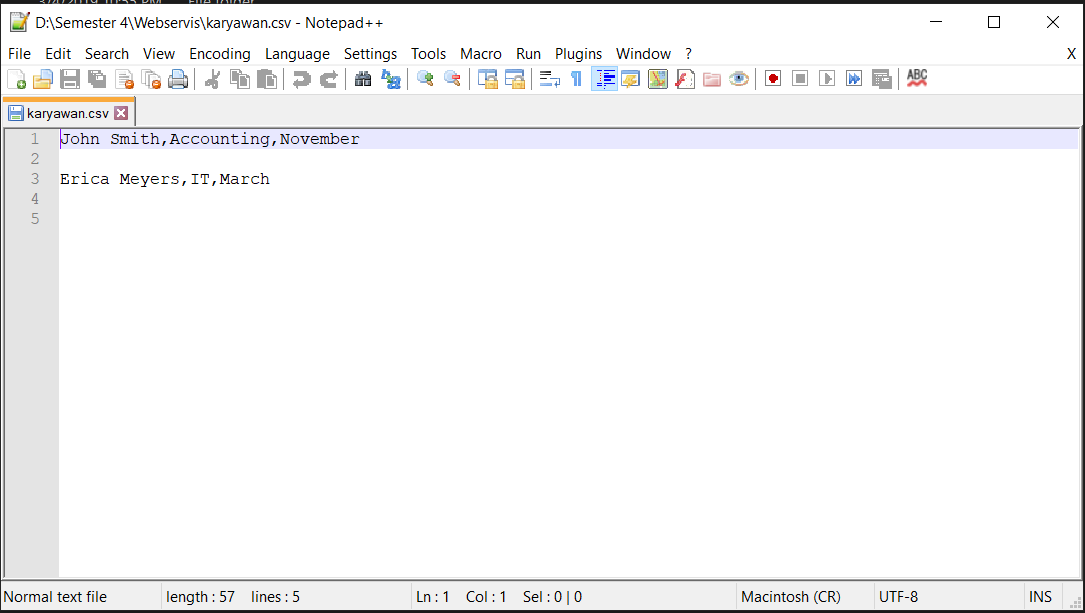
\includegraphics[width=0.5\textwidth]{figures/chapter4/1174040_csv.png}}
            \caption{Contoh CSV}
            \label{1174040_csv}
            \end{figure}

	\item Ms.Excel , NotePad, notepad++, sublime, dan texteditor lainnya

	\item caranya adalah :
		\begin{itemize}
			\item untuk write :
			\begin{enumerate}
				\item Download template csv
				\item Buka browser lalu menuju ke Google Sheet
				\item Tekan tombol merah di pojok kanan bawah
				\item Lalu pilih upload file untuk mengupload template yang sudah di download sebelumya
				\item Edit sesuai yang diinginkan
				\item Setelah selesai, lalukan eksport ke CSV dengan cara klik file lalu download as setelah itu pilih CSV
			\end{enumerate}
			\item untuk read :
			\begin{enumerate}
				\item buka Ms.Excel
				\item pilih Data lalu Get External Data dan pilih From Text
				\item lalu pilih file csv nya
				\item pilih Delimeted lalu Next
				\item checklist di box Tab dan Comma
				\item lalu klik finish
			\end{enumerate}
		\end{itemize}	
	\item Library CSV berisikan fungsi -fungsi dan kelas yang akan dipakai dalam pengerjaan file CSV

	\item Pandas diciptakan pada tahun 2008 oleh Wes McKinney dan diperbaharuin pada tahun 2010 oleh Sien Chang. yang fungsinya untuk melakukan analisa data seperti import dan export data.

	\item Fungsi - funsi library csv adalah :
		\begin{itemize}
			
			\item \begin{verbatim}csv.reader(csvfile, dialect='excel', **fmtparams)\end{verbatim} : digunakan untuk membaca line di csv
			\item \begin{verbatim}csv.writer(csvfile, dialect='excel', **fmtparams)\end{verbatim} : untuk menulis line di csv
			\item \begin{verbatim}csv.register_dialect(name[, dialect[, **fmtparams]]) \end{verbatim}: untuk asosiasikan dialect dengan name, dimana name harus string
			\item \begin{verbatim}csv.unregister_dialect(name)\end{verbatim} : menghapus dialect yang terasosiasi dengan name
			\item \begin{verbatim}csv.get_dialect(name)\end{verbatim} : mengnembalikan hasil dialect yang terasosisasi dengan name
			\item \begin{verbatim}csv.list_dialects() \end{verbatim}: menampilkan semua dialect yang ada
			\item \begin{verbatim}csv.field_size_limit([new_limit])\end{verbatim} : menamplikan field maksimal ayng di berikan oleh pembubat parse.

		\end{itemize}

	\item Pandas mengngunakan sistem dataframe yang memeprbolehkan kita untuk memasukkan sebuah file ke dalam tabel vitual seperti spreadsheet.kita dapat mengolah dengan fungsi - fungsi  seperti join, distinct, group by, agregasi dan funsi lain seperti dalam SQL tetapi dibuat pada tabel yang dimuat di file ke ram
	\end{enumerate}

\section{IrvanRizkiansyah/1174043}
	\subsection{Pemahaman Teori}
		\begin{enumerate}
			\item \begin{itemize}
					\item Fungsi : File csv berfungsi untuk pencarian data akan menjadi lebih mudah dan cepat, dan juga mempermudah penginputan data ke dalam database secara sederhana.
					\item Sejarah : File csv muncul pertama kali sekitar 10 tahun sebelum Personal Computer (PC) pertama  didunia yaitu sejak sekitar tahun 1972, akan tetapi sebutan file csv digunakan pertama kali pada tahun 1983.
					\item Contoh : 
						\begin{figure} [ht]
							\centerline{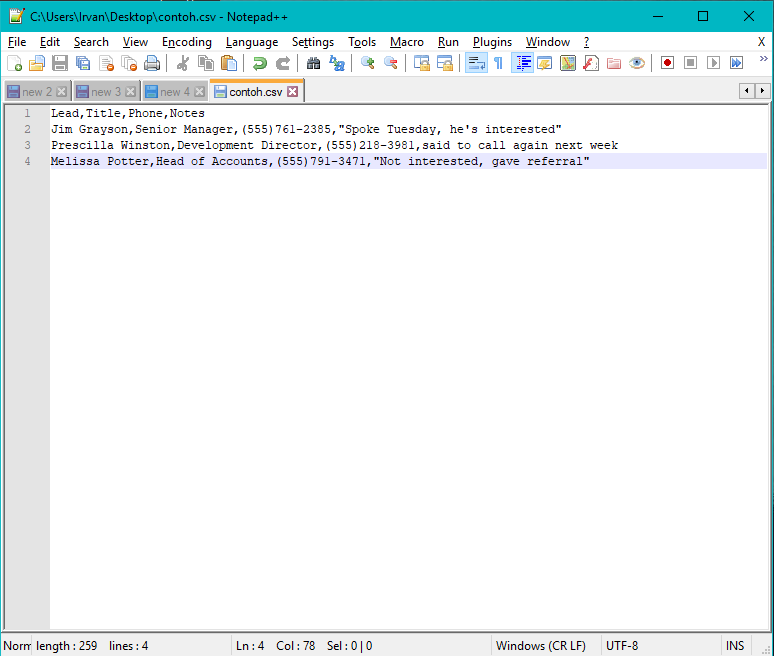
\includegraphics[width=0.6\textwidth]{figures/chapter4/Contoh_CSV.png}}
							\caption{Contoh CSV}
							\label{Contoh CSV}
						\end{figure}

					\ref{Contoh_CSV}
				\end{itemize}
			
			\item Ada banyak aplikasi yang dapat membuat file berformat CSV, diantaranya adalah :
				\begin{itemize}
					\item Notepad
					\item Notepad++
					\item Microsoft Excel
					\item Corel Quatro Pro
					\item Apache Open Office, dan masih banyak yang lainnya.
				\end{itemize}
			
			\item Cara menulis file csv menggunakan Excel :
				\begin{enumerate}
					\item Buka aplikasi Microsoft Excel kemudian buat dokumen baru
					\item Tulis judul kolom untuk setiap informasi yang ingin di rekam atau catat, kemudian tulis informasi - informasi dalam kolom dengan sesuai.
					\item Jika sudah selesai maka save dengan cara pilih menubar File lalu pilih Save As
					\item Lalu isikan nama file tersebut dan rubah dengan memilih format file yang tersedia tersebut menjadi .csv
					\item File csv sudah berhasil terbuat menggunakan Microsoft Excel
				\end{enumerate}
			\item Cara membaca file csv menggunakan Excel :
				\begin{enumerate}
					\item Buka aplikasi Microsoft Excel kemudian pilih menu Open
					\item Cari tempat file csv yang ingin dibuka, kemudian pilih Open
					\item File csv sudah berhasil dibaca menggunakan Microsoft Excel
				\end{enumerate}
			
			\item Pada file csv, tanda baca koma diartikan sebagai pembatas suatu kolom. List-directed input output didefinisikan dalam FORTRAN 77. List-directed input menggunakan tanda baca koma atau spasi sebagi pembatas, sehinnga karakter yang tidak dikutip tidak dapat mengandung tanda baca koma ataupun spasi. Hal tersebut yang diadopsi oleh file csv. format csv didukung dengan library untuk banyak bahasa pemrograman, kebanyakan yang menspesifikasikan pembatas field, pemisah desimal, pengkodean karakter, dan yang lainnya.
			
			\item Pada tahun 2008, pengembangan pandas dimulai oleh AQR Capital Management. Pada akhir tahun 2009 pandas menjadi Open Sourced, dimana disupport oleh banyak komunitas atau individu di dunia untuk mengembangkan pandas. Sejak tahun 2015, pandas menjadi NumFOCUS proyek sponsor, ini juga membantu suksesnya pengembangan dari pandas itu sendiri. pandas merupakan struktur data dan data analysis tools untuk bahasa pemrograman Python, dan merupakan BSD-licensed library yang menjadikannya memiliki performa yang tinggi.
			
			\item 
				\begin {itemize} 
					\item Tanda baca koma : Menjadi pemisah antar kolom
					\item Tanda baca kutip dua : Menjadi cara untuk memasukan sebuah kalimat atau untuk memasukan karakter spasi sebagai data pada kolom informasi
					\item Inputan pada baris pertama akan menjadi Header, dimana akan menjadi nama sebuah kolom, dan masih banyak yang lainnya
				\end{itemize}
			
			\item Pada pandas sedikit berbeda, dimana inputan data berbentuk seperti peng-inputan pada variabel pada umumnya, hanya saja menggunakan tanda kutip satu untuk menandakan sebuah informasi pada kolom kemudian tanda kurung kotak yang didalamnya berisi informasi data dari kolom tersebut. dan lain sebagainya.
			
		\end{enumerate}

\subsection{Luthfi Muhammad Nabil/1174035}
\subsubsection{Fungsi, Sejarah, dan Contoh file CSV}
\begin{itemize}
	\item Fungsi \linebreak File CSV (Comma Separated Values) adalah tipe file khusus yang menyimpan informasi dengan metode dipisahkan dengan koma. File CSV berfungsi untuk menjadi perantara untuk beberapa aplikasi yang memiliki basis data saat mengirim data. CSV dapat dibuka di berbagai text editor
	yang ada. Dengan bentuk filenya yang dinamis memungkinkan file CSV dapat dimanipulasi dan dapat menyimpan informasi dengan skala besar.
	\item Sejarah \linebreak CSV sudah digunakan sejak tahun 1972 yang dapat dikompilasi pada bahasa pemrograman IBM Fortran. Saat itu, data yang dipisahkan oleh koma jika isinya memiliki spasi maka harus diberi tanda petik di awal dan akhir isi dari data tersebut. Nama CSV baru mulai digunakan pada tahun 1983. Pada panduan dari Osborne Executive Computer mendokumentasikan kutipan yang membolehkan isi karakter memiliki koma.  Pada tahun 2005 dengan RFC4180, CSV didefinisikan sebagai MIME Content Type. lalu pada tahun 2013, defisiensi dari RFC4180 dipecahkan oleh rekomendasi dari W3C. Pada tahun 2014, IETF mempublikasi RFC7111 yang mendeskripsikan pecahan Uniform Resource Identifier(URI) ke dokumen CSV. RFC7111 menjelaskan bagaimana baris, kolom dapat dipilih dalam dokumen CSV menggunakan indeks posisi. Pada Tahun 2015, W3C mempublikasikan draft rekomendasi untuk CSV-metadata standards yang dimulai dengan rekomendasi pada bulan Desember dengan tahun yang sama. 
	\item Contoh File CSV \begin{itemize}
							\item 
							CSV pada Excel \ref{1174035_CSVExcel}
							\begin{figure}[!htbp]
								\centering
								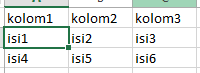
\includegraphics[height=4cm, width=7cm]{figures/chapter4/1174035_CSVExcel.jpg}
								\caption{Contoh CSV Pada Excel}
								\label{1174035_CSVExcel}
							\end{figure}
							\item \begin{figure}[!htbp]
								\centering
								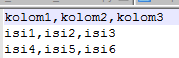
\includegraphics[height=4cm, width=7cm]{figures/chapter4/1174035_CSVText.jpg}
								\caption{Contoh CSV Pada Text}
								\label{1174035_CSVText}
							\end{figure}
							CSV pada Text Editor \ref{1174035_CSVText}
							
						  \end{itemize}
\end{itemize}
\subsubsection{Aplikasi Yang dapat membuat file CSV}
Berikut file yang dapat membuat file CSV
\begin{itemize}
	\item Spreadsheet \linebreak Spreadsheet merupakan aplikasi yang dapat membuat CSV hanya dengan memasukan data sesuai baris dan kolom yang diinginkan. Contoh spreadsheet seperti Google Spreadsheet, Microsoft Excel, dan aplikasi lainnya. 
	\item Bahasa Pemrograman \linebreak Bahasa pemrograman merupakan media yang dapat untuk membuat aplikasi yang dapat membuat file CSV khusus untuk bahasa pemrograman yang support dengan pembuatan file CSV. Seperti Python, C Sharp, dan lain sebagainya.
	\item Text Editor \linebreak Text editor juga dapat membuat file CSV, untuk membuat dengan Text Editor cukup dengan membuat file sesuai format CSV dan save file tersebut dengan ekstensi .CSV.
\end{itemize}
\subsubsection{Menulis dan Membaca file CSV}
Berikut cara menulis dan membaca file CSV : 
\begin{itemize}
	\item Menulis : \begin{enumerate}
						\item Buka file CSV dengan spreadsheet
						\item Klik Cell yang mau diisi
						\item Masukan data yang mau diisi pada cell tersebut
						\item Lalu save file dengan format .CSV
					\end{enumerate}
	\item Membaca : \begin{enumerate}
						\item Buka file CSV dengan spreadsheet						
					\end{enumerate}
\end{itemize}
\subsubsection{Sejarah Library CSV Python}
Library CSV pada python merupakan library yang paling umum untuk import export data pada spreadsheet dan basis data dengan format sesuai dengan standarisasi RFC4180. Seiring dengan lahirnya bahasa pemrograman python, library mulai dibuat dan dikembangkan sampai akhirnya pada tahun 2003, pembuatnya Kevin Altis dan lainnya telah merilis versi final untuk library Python CSV. 
\subsubsection{Sejarah Library Pandas Python}
Pandas (Python Data Analysis Library) adalah library open source yang digunakan untuk melakukan data manajemen dan data analysis. Pandas diciptakan pada tahun 2008 oleh Wes McKinney dan diperbaharui oleh Sien Chang pada tahun 2010. Inspirasi dari pembuatan pandas muncul pada komunitas yang membutuhkan library khusus untuk analisis data. 
\subsubsection{Fungsi - fungsi yang terdapat di library CSV}
\begin{itemize}
	\item \begin{verbatim} csv.reader(csvfile, dialect='excel', **fmtparams) \end{verbatim} Untuk mengembalikan	object reader yang akan mengambil setiap line pada csv yang diambil. Data setiap baris diambil saat next() dipanggil. Berikut contohnya : \lstinputlisting[firstline=1, lastline=6]{src/chapter4/chap4_1174035_teori.py}
	\item \begin{verbatim} csv.writer(csvfile, dialect='excel', **fmtparams) \end{verbatim} Mengembalikan file pembuat object untuk dapat mengkonversi data pada python ke file CSV yang akan dibuat. Berikut contoh penggunaan csv.writer : \lstinputlisting[firstline=8, lastline=14]{src/chapter4/chap4_1174035_teori.py}
	\item \begin{verbatim} csv.register_dialect(name[, dialect[, **fmtparams]]) \end{verbatim} Mengasosiasikan dialek dengan nama, nama yang dimasukkan harus berupa karakter.
	\item \begin{verbatim} csv.unregister_dialect(name) \end{verbatim}
	Menghapus asosiasi dialek dengan nama pada registry dialek.
	\item \begin{verbatim} csv.get_dialect(name) \end{verbatim}
	Mengambil dialek yang telah diasosiasikan dengan nama. 
	\item \begin{verbatim}  csv.list_dialects() \end{verbatim} Mengembalikan dialek yang telah diregistrasi.
	\item \begin{verbatim} csv.field_size_limit([new_limit]) \end{verbatim} Mengembalikan maksimal kolom data yang diperbolehkan oleh pembaca.
\end{itemize}
\subsubsection{Fungsi - fungsi yang terdapat di library Pandas}
\begin{itemize}
	\item \begin{verbatim} pandas.read_csv(filepath_or_buffer[, sep, …]) \end{verbatim} Untuk membaca file CSV dan menyimpannya ke DataFrame
	\item \begin{verbatim} pandas.read_excel(io[, sheet_name, header, names, …])  \end{verbatim} Membaca file excel dan menyimpannya ke DataFrame
	\item \begin{verbatim} to_csv([path, index, sep, na_rep, …]) \end{verbatim}
	Untuk membuat file CSV dari data yang ada	
\end{itemize}

\section{Faisal Najib Abdullah}
\subsection{Pemahaman Teori}
\begin{enumerate}
    \item Apa itu fungsi file csv, jelaskan sejarah dan contoh ?
    \par
    File CSV Nilai Berbatas Koma adalah tipe file khusus yang dapat Anda buat atau edit di Excel. File CSV menyimpan informasi yang dipisahkan oleh koma, bukan menyimpan informasi dalam kolom. Saat teks dan angka disimpan dalam file CSV, mudah untuk memindahkannya dari satu program ke program lain.
    \par 
	File CSV dibuat oleh program yang menangani sejumlah data yang besar. CSV merupakan cara yang nyaman untuk mengekspor data dari spreadsheet dan basis data serta mengimpor atau menggunakannya dalam program lain. Misalnya, Anda dapat mengekspor hasil program penambangan data ke file CSV dan kemudian mengimpornya ke dalam spreadsheet untuk menganalisis data, menghasilkan grafik untuk presentasi, atau menyiapkan laporan untuk publikasi.
    \par
	Contohnya, Anda dapat mengekspor kontak dari Google ke dalam file CSV, kemudian mengimpornya ke Outlook.
    
    \item Aplikasi-aplikasi apa saja yang bisa menciptakan file csv?
    Pada Windows
    \begin{itemize}
        \item Microsoft Excel 2013
        \item Microsoft Works
        \item CCorel Quattro Pro
        \item Apache OpenOffice
        \item LibreOffice
        \item Microsoft Notepad
        \item Intuit Quicken 2015
        \item GenScriber
    \end{itemize}
    Pada Mac OS
    \begin{itemize}
        \item Microsoft Excel 2011
        \item Planamesa NeoOffice
        \item Apache OpenOffice
        \item LibreOffice
        \item GenScriber
    \end{itemize}
    Pada Linux
    \begin{itemize}
        \item Apache OpenOffice
        \item LibreOffice
        \item GenScriber
    \end{itemize}
    
    \item Jelaskan bagaimana cara menulis dan membaca file csv di excel atau spreadsheet?
	\begin{itemize}
        \item Cara menulis file csv harus berupa baris dan kolom atau bisa juga di sebut berupa tabel.
        \item Untuk membacanya file csv dipisahkannya menggunakan koma atau titik koma.
    \end{itemize}
    
    \item Jelaskan sejarah library csv?
	Library csv menyediakan fungsionalitas untuk membaca dan menulis ke file CSV. Dirancang untuk bekerja di luar kotak dengan file CSV yang dihasilkan Excel, memudahkan untuk bekerja dengan berbagai format CSV. Library csv berisi objek dan kode lain untuk membaca, menulis, dan memproses data ke file CSV.
    
    \item Jelaskan sejarah library pandas?
	panda adalah pustaka Python open-source yang menyediakan alat analisis data kinerja tinggi dan struktur data yang mudah digunakan. panda tersedia untuk semua instalasi Python, tetapi itu adalah bagian penting dari distribusi Anaconda dan bekerja sangat baik di notebook Jupyter untuk berbagi data, kode, hasil analisis, visualisasi, dan teks naratif.

    \item Jelaskan fungsi-fungsi yang terdapat di library csv?
	Terdapat 2 fungsi yang bisa digunakan oleh library csv
    Pertama,fungsi membaca file csv.
    fungsi ini bisa menggunakan list dan dictionary
    Dengan list :
    \lstinputlisting[firstline=11, lastline=21]{src/chapter4/1174042_csv.py}
    Dengan dictionary :
    \lstinputlisting[firstline=24, lastline=33]{src/chapter4/1174042_csv.py}
    Kedua,fungsi menulis file csv.
    \lstinputlisting[firstline=36, lastline=40]{src/chapter4/1174042_csv.py}
    
    \item Jelaskan fungsi-fungsi yang terdapat di library pandas
	Hampir sama dengan library csv,tp library pandas penulisannya lebih sederhana dan terlihat lebih rapih dari pada library csv.
    \lstinputlisting[firstline=43, lastline=44]{src/chapter4/1174042_csv.py}
    

\end{enumerate}

\section{Fathi Rabbani / 1164074}
\subsection{Teori}
\begin{enumerate}
\item Sejarah dan Penjelasan CSV
\subitem Penggunaan dari format file CSV itu sendiri untuk memudahkan pembuatan data dengan menggunakan tanda koma sebagai pembatas dari datanya agar mudah untuk dibaca pada kolom.
\subitem CSV sendiri dibuat untuk dapat menangani pembuatan sejumlah data yang berukuran besar, mempermudah program dalam membaca datanya kedalam kolom - kolom. seperti contoh dalam membacanya menggunakan aplikasi Excel sehingga mempermudah dalam proses import dan eksport datanya. csv sendiri sudah ada pada tahun 1972 dengan pengembangnya adalah IBM namun penggunaannya masuk pada tahun 1983 yang berbarengan dengan adanya SuperCalc spreadsheet.

\item Aplikasi CSV
\begin{itemize}
\item Microsoft Excel
\item Open Office Calc
\item Google Docs
\item Libre Office
\item Apache Open Office
\end{itemize}

\item Menulis dan Membaca csv di Excel atau Spreadsheet
\subitem Menulis, cara menuliskan csv adalah dengan menggunakan tanda baca koma pada bagian data yang ingin dipisah contohnya \lstinputlisting[firstline=8, lastline=29]{src/chapter4/coba.csv}
\subitem Membaca, file csv dapat dibaca pada program aplikasi Excel dengan menampilkan hasil data dari setiap data yang dipisah dengan tanda baca koma menjadi kolom - kolom hasilnya ada pada \ref{fig1}

\item Library CSV
\subitem CSV atau comma separated value adalah salah satu tipe file yang digunakan secara luas di dunia programming. Tidak hanya itu CSV pun sering digunakan dalam pengolahan informasi yang dihasilkan spreadsheet untuk diproses lebih lanjut melalui mesin analitik. CSV pun dianggap sebagai file yang agnostik karena dapat digunakan oleh berbagai database untuk proses backup data.

\item Library Pandas
\subitem pandas merupakan library pada pemrograman python yang berguna untuk mengolah dan meyediakan struktur data serta analisa data yang mudah untuk dibaca dan dipahami seperti pada struktur data tabel. pandas dapat melakukan proses perbandingan data, penggabungan dataset, penanganan dataset yang hilang dll. pandas dapat juga digunakan sebagai pemrosesan data Statistik dengan pembacaan datanya menggunakan struktur Spreadsheet.

\item Fungsi pada Library CSV
\begin{itemize}
\item Menulis data CSV
\lstinputlisting[firstline=8, lastline=29]{src/chapter4/coba.csv}
\item Hasil dari menullis data CSV
\lstinputlisting[firstline=31, lastline=37]{src/chapter4/coba.csv}
\item Membaca data CSV
\lstinputlisting[firstline=40, lastline=52]{src/chapter4/coba.csv}
\item Hasil pembacaan data CSV
\lstinputlisting[firstline=54, lastline=60]{src/chapter4/coba.csv}
\end{itemize}

\item Fungsi pada Library Pandas
\begin{itemize}
\item Kode
\lstinputlisting[firstline=62, lastline=67]{src/chapter4/coba.csv}
\item Hasil
\lstinputlisting[firstline=69, lastline=73]{src/chapter4/coba.csv}
\end{itemize}
\end{enumerate}

\begin{figure}[!htbp]
	\centering
	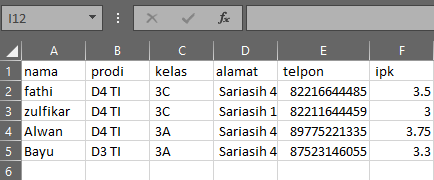
\includegraphics[width=1\textwidth]{figures/chapter4/1164074/1}
	\caption{hasil csv pada Excel}
	\label{fig1}
\end{figure}

\section {Kevin Natanael Nainggolan 1174059}
	\begin {enumerate}
		\item Apa itu fungsi csv, jelaskan sejarah dan contohnya 
			\lstinputlisting [firstline=10, lastline=14]{src/teoric4.py}
		\item Aplikasi-aplikasi apa saja yang bisa menciptakan file csv? 
			\lstinputlisting [firstline=18, lastline=22]{src/teoric4.py}
		\item Jelaskan bagaimana cara menulis dan membaca file csv di excel atau spreadsheet
			\lstinputlisting [firstline=26, lastline=39]{src/teoric4.py}
		\item Jelaskan sejarah library csv
			\lstinputlisting [firstline=43, lastline=50]{src/teoric4.py}
		\item Jelaskan sejarah library pandas
			\lstinputlisting [firstline=54, lastline=60]{src/teoric4.py}
		\item Jelaskan fungsi-fungsi yang terdapat di library csv
			\lstinputlisting [firstline=64, lastline=68]{src/teoric4.py}
		\item Jelaskan fungsi-fungsi yang terdapat di library pandas
			\lstinputlisting [firstline=72, lastline=75]{src/teoric4.py}
	\end {enumerate}

\section{Yusniar Nur Syarif Sidiq/1164089}
\subsection{Pemahaman Teori}

\begin{enumerate}

\item Apa itu fungsi file csv, jelaskan sejarah dan contoh.
	\subitem File csv merupakan jenis file khusus yang dapat kita buat dan edit di dalam Excel. File csv akan menyimpan informasi data yang dipisahkan dengan koma atau tanda titik koma, dimana artinya file csv tidak menyimpan data dalam bentuk kolom. Saat pertama kali rilis, excel menggunakan format file dalam bentuk biner yaitu BIFF sebagai format file utama. Namun setelah Microsoft merilis Ofice System 2007, Excel telah menggantikan format utamanya menjadi XML. Meskipun mendukung format XML baru, Excel masih mendukung format BIFF, tidak hanya itu excel juga telah mendukung format CSV, DBF, SYLK, DIF, dan format-format lainnya. Fungsi dari file csv itu sendiri adalah mempermudah dalam pencarian data dan pengimputan data ke dalam database sederhana. File csv mulai digunakan pada tahun 1983 akan tetapi format file csv sudah ada dari tahun 1972. Contoh file dengan format csv dapat dilihat pada figure \ref{YNCSV1}

	\begin{figure}[ht]
		\centering{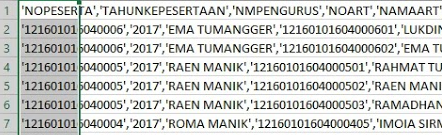
\includegraphics[scale=0.5]{figures/chapter4/YN/Chapter4/YNCSV1.png}}
		\caption{Contoh File CSV}
		\label{YNCSV1}
	\end{figure}

\item Aplikasi - aplikasi apa saja yang bisa menciptakan file csv.
	\subitem Untuk membuat file dengan format CSV, kita dapat menggunakan software bawaan Microfsoft Ofice yaitu Excel. Bukan hanya Microsoft Excel, kita juga dapat membuat file CSV dengan bantuan text editor. Jika kita ingin membuat file csv secara online dapat menggunakan Google Spreadshare. Apabila OS PC kita menggunakan Linux dapat menggunakan LibreOfficecalc.

\item Jelaskan bagaimana cara menulis dan membaca file csv di excel atau spreadsheet.
	\subitem Cara membuat file CSV dengan Excel
			\begin{itemize}
				\item Buka software Microsoft Excel
				\item Pilih new document
				\item Buatlah judul kolom yang ingin kita rekam
				\item Isikan informasi - informasi pada setiap kolom
				\item Simpan dengan menggunakan metode save as
				\item Cari dan pilih format csv
				\item Pilih button save untuk melakukan penyimpanan
			\end{itemize}
	\subitem Cara membaca file CSV dengan Excel
			\begin{itemize}
				\item Buka software Microsoft Excel
				\item Lakukan perintah open file
				\item Cari file csv yang sudah kita buat sebelumnya
				\item Pilih button open untuk membaca file csv pada Microsoft Excel
			\end{itemize}
	\subitem Cara membaca file csv dari Excel
		\lstinputlisting[firstline=1, lastline=9]{src/chapter4/1164089.py}
	\subitem Cara membuat file csv
		\lstinputlisting[firstline=12, lastline=16]{src/chapter4/1164089.py}

\item Jelaskan sejarah library csv. 
	\subitem Pada tahun 1972 adalah terbentuknya format file csv namun bukan hanya itu saja, pada saat itupun terbentuk juga yang namanya library pandas.Seiring dengan lahirnya bahasa pemrograman python, library mulai dibuat dan dikembangkan oleh Kevin Altis. Dengan kata lain CSV dibentuk pada tahun 1972 dan sudah satu paket baik dalam librarynya maupun format filenya. 

\item Jelaskan sejarah library pandas.
	\subitem Developer yang bernama Wes McKinney telah mengajarkan pandas pada tahun 2008 ketika ia berada di AQR Capital Management, karena kebutuhan akan alat kinerja tinggi yang fleksibel untuk melakukan analisis kuantitatif pada data keuangan. Sebelum meninggalkan AQR, dia dapat meyakinkan manajemen untuk mengizinkan membuka sumber library. Pegawai AQR lainnya yaitu Chang She, telah bergabung dengan upaya ini pada 2012 sebagai kontributor utama kedua ke library. Pada tahun 2015, pandas telah menandatangani sebagai proyek NumFocus yang disponsori secara fiskal. Pada saat itulah Library Pandas mulai berjalan dan digunakan.

\item Jelaskan fungsi-fungsi yang terdapat di library csv.
	\subitem Ada dua fungsi pada library csv, yaitu csv.reade dan csv.writer. Dimana fungsi tersebut memiliki tugas yang berbeda-beda. Untuk csv.reader bertugas sebagai membaca file csv sedangkan csv.writer bertugas membuat file csv.

\item Jelaskan fungsi-fungsi yang terdapat di library pandas.
	\subitem Untuk library pandas sama saja dengan library csv namun bedanya hanya cara penulisan source codenya saja. Untuk membaca file csv pada library pandas membutuhkan perintah pandas.read\_csv sedangkan untuk membuat file csv membutuhkan perintah pandas.write\_csv.

\end{enumerate}



\bibliographystyle{IEEEtran} 
%\def\bibfont{\normalsize}
\bibliography{references}


%%%%%%%%%%%%%%%
%%  The default LaTeX Index
%%  Don't need to add any commands before \begin{document}
\printindex

%%%% Making an index
%% 
%% 1. Make index entries, don't leave any spaces so that they
%% will be sorted correctly.
%% 
%% \index{term}
%% \index{term!subterm}
%% \index{term!subterm!subsubterm}
%% 
%% 2. Run LaTeX several times to produce <filename>.idx
%% 
%% 3. On command line, type  makeindx <filename> which
%% will produce <filename>.ind 
%% 
%% 4. Type \printindex to make the index appear in your book.
%% 
%% 5. If you would like to edit <filename>.ind 
%% you may do so. See docs.pdf for more information.
%% 
%%%%%%%%%%%%%%%%%%%%%%%%%%%%%%

%%%%%%%%%%%%%% Making Multiple Indices %%%%%%%%%%%%%%%%
%% 1. 
%% \usepackage{multind}
%% \makeindex{book}
%% \makeindex{authors}
%% \begin{document}
%% 
%% 2.
%% % add index terms to your book, ie,
%% \index{book}{A term to go to the topic index}
%% \index{authors}{Put this author in the author index}
%% 
%% \index{book}{Cows}
%% \index{book}{Cows!Jersey}
%% \index{book}{Cows!Jersey!Brown}
%% 
%% \index{author}{Douglas Adams}
%% \index{author}{Boethius}
%% \index{author}{Mark Twain}
%% 
%% 3. On command line type 
%% makeindex topic 
%% makeindex authors
%% 
%% 4.
%% this is a Wiley command to make the indices print:
%% \multiprintindex{book}{Topic index}
%% \multiprintindex{authors}{Author index}

\end{document}
